\subsection{Tipi di controlli}

La vulnerabilità è ciò che una minaccia sfrutta per portare un attacco.

\paragraph*{Tolleranza zero}
La tolleranza zero è una policy adottata all'interno dell'azienda, su cui
l'azienda di solito non transige ed esegue il licenziamento. Alcuni esempi sono
per esempio su discriminazioni raziali o basati sulla religione.

\begin{figure}[H]
 \centering
 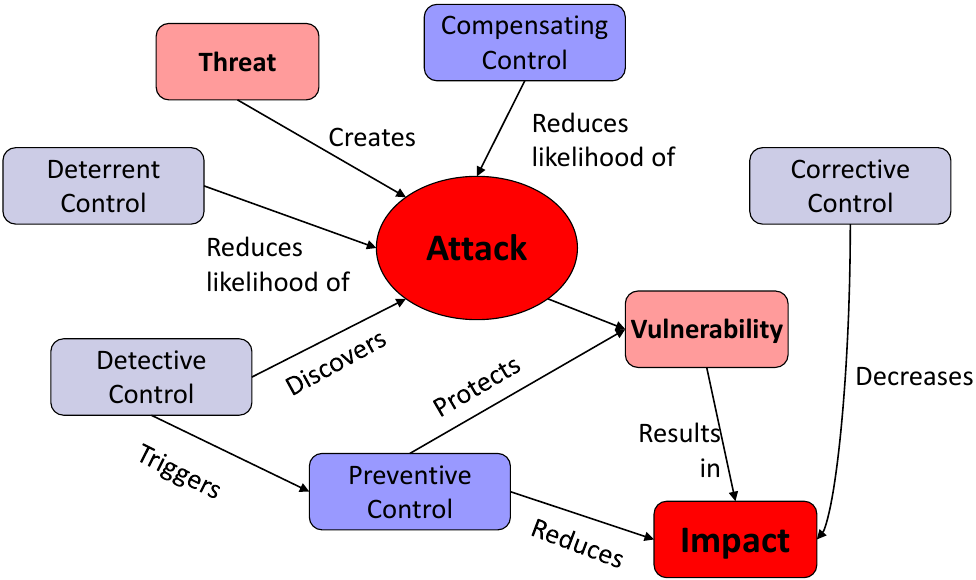
\includegraphics[scale=0.5]{controlTypes}
 \caption{Schema dei diversi tipi di controlli}
\end{figure}



\paragraph*{Controlli e contromisure}

Il costo del controllo non dovrebbe mai superare la perdita attesa.
Una contromisura la si può vedere come un controllo mirato (specifico per un
particolare tipo di minaccia o vulnerabilità)

\paragraph*{Monitoraggio del rischio}

Praticamente consiste nel PDCA\footnote{Ciclo di Deming}.
C'è l'IOS\footnote{Office of Internal IOS Service è l'ufficio che se ne occupa.}
che fa il planning dell'audit per i prossimi $n$ anni.


\paragraph*{Security control baselines and metrics}

Una \textit{baseline} è un parametro di riferimento ed è molto importante,
perchè ci permette di prendere le misure sulle cose per vedere se stiamo
migliorando o meno!
Le misure sono collezionate durante gli anni. La consistenza delle misurazioni
sono molto importanti.

\section{Risk management}

È un qualcosa che dev'essere allineato con la strategia aziendale.
È business driven (non technology driven).

Lo \textit{steering committee} definisce le proprietà della gestione del rischio.
Ed è preferibile metterci gente che conosce a fondo il business.

\subsection{I ruoli del risk-management}

I ruoli del \textit{risk management} sono:
\begin{itemize}
\item CIO e CISO\footnote{La tendenza è quella di fondere i ruoli};
\item Security Trainers: sono sostanzialmente dei consulenti, e sono incaricati
di sviluppare materiale d'insegnamento adeguato per educare gli utenti finali
\item System/Info Owners: responsabili di assicurarsi che i controlli siano
funzionanti;
\item Governance and Security Management: allocano risorse, valutano e usano i
risultati della valutazione del rishio;
\item Business Managers: prendono decisioni difficili riguardo alla priorità
di raggiungere i \textit{business goals};
\item IT Security Practitioners: implementano la sicurezza nei sistemi IT.
\end{itemize}

\subsection{Due Diligence}

È quella cosa che va messa in piedi per non essere perseguiti in maniera civile,
ovvero far le cose con ``buon senso''. Oggi come oggi si esegue il \textit{risk
assessment} per prevenire guai dal punto di vista civile. La \textbf{due care}
si esegue per ridurre il rischio a livelli accettabili. Nell'ordinamento
giuridico italiano il termine è diligenza del buon padre di famiglia (articolo
1176).


\section{Esercizi}

Gli esercizi relativi a questa parte si possono trovare in \ref{esGestRisk}
